
\chapter{Introduction}


\section{Quantum Computing}
The computer age started in 1936 when A. M. Turing invented the first computer, which also bore his name. This computer led not only science, but arguably every aspect of life down an accelerated route to improvement due to the computational advantage that it gave. A new revolution began in 1980 through the work of Manin \cite{Manin1980}, when he described a new type of computing: Quantum Computing. 
\\\\ 
Different algorithms or problems can be attributed a level of complexity based on the time, or steps, it takes a machine to solve a problem in relation to the size of the problem. The main classes of interest are whether a problem scales exponentially with the problem size (inefficient to compute) or whether it scales polynominally with the problem size(efficient to compute).

The utility of quantum computing stems from a point made by Deutsch inn 1985 \cite{Deutsch1985}, that a problem need not have the same level of complexity when solved on different types of machines. This means that a problem which is difficult to solve on a Turing machine, may not be difficult to solve on another type of machine (such as a quantum computer). This point was confirmed in 1994 when Shor discovered the Fast Fourier Transformation Algorithm for quantum computers  \cite{Shor1994}; as the first example of an algorithm that is faster to solve on a quantum computer. This algorithm's use in compromising the security of public key encryption techniques greatly increased interest in quantum computing.
Since then, new algorithms with improved speed have been discovered for quantum computing. As these new algorithms are discovered, the utility of quantum computers increases. 
\\\\
The key component of a quantum computer is a new type of information, called the qubit. Qubits are physically realized by any two level quantum system. The state of a qubit can be described by the state $\ket{\alpha}$, in equation \ref{eq:qubit}.
\begin{align}
\ket{\psi} = \alpha\ket{0} + \beta\ket{1}\\
|\alpha|^2+|\beta|^2 = 1	
\label{eq:qubit}
\end{align}
Where $\alpha,\beta\in \textbf{C}$. For a qubit, the global phase is unobservable, while the local phase is observable. For this reason, we can make the simplification that $\alpha \in \textbf{R}, \beta \in \textbf{C}$.
\subsection*{Pure Vs. Mixed States}
The qubit takes a linear superposition of the base kets $\ket{0}$ and $\ket{1}$, to represent its state of $\ket{\psi}$. When the qubit is measured, its superposition will collapse onto one of the base kets, and an eigenvalue of one of the base kets will be measured with probabilities determined by $P(\alpha)=|\alpha|^2$ and $P(\beta)=|\beta|^2$. This is not to say that the qubit is ever actually in one of the states $\ket{0}$ or $\ket{1}$ before being measured (it is in fact in the state $\ket{\psi}$), but rather to say that the base kets are what state it is in \textbf{after} being measured, due to the measurement projecting onto the base kets. The base kets are simply a way to describe the state of the system. This describes the measurement of a \textit{pure state}. For a \textit{mixed state}, (which can be created through error processes) the measurement outcomes can appear similar, but they are two distinct cases. The uncertainty in measurement you get from a mixed state comes from uncertainty in the density matrix, whereas a pure state in a superposition has no uncertainty in it's density matrix; its uncertainty in measurement outcomes comes from the projective measurement made on the superposition. It is important to note that a mixed state is constituted of multiple pure states, and those states can be in a superposition of states; leading to 2 levels of uncertainty (one classical, and one quantum)
\\\\
For the base kets $\ket{0}$ and $\ket{1}$, there is a standard basis that is used. 
\[
\ket{0} = 
\begin{bmatrix}
1 \\
0 
\end{bmatrix},
\ket{1} = 
\begin{bmatrix}
0 \\
1 
\end{bmatrix}
\]
\\\\
As with any quantum system, it is difficult to isolate a quantum computer from its environment. This interaction causes the quantum state of the particles constituting the computer to decohere, introducing errors. 
The decoherance of the system is known as an error channel. Thus for a density matrix $\rho = \ket{\psi}\bra{\psi}$ we have;
$$\xi (\rho) = U\rho U^\dagger $$
where $U$ is some quantum operation. The general error channel is the Pauli channel shown in equation \ref{eq:pauli}\footnote{conjugates are hidden, as Pauli operators are Hermetian operators}.
\begin{equation}
\xi(\rho) = (1-P_X-P_Y-P_Z)\rho +P_XX\rho X+P_YY\rho Y +P_ZZ\rho Z
\label{eq:pauli}
\end{equation}
X, Y and Z refer to the Pauli matrices\footnote{see appendix \ref{app:pauli}}, and $P_X$, $P_Y$ and $P_Z$ refer to the probabilities of X, Y and Z errors occurring respectively.
\\\\
This Pauli channel says that any error on a qubit can be represented as a linear combination of no errors (I), Bit Flip Errors (X), Phase Errors (Z) and Bit Flip Phase Errors (Y). 

Thus, an error on a prepared state $\ket{\Psi}$ can be represented by:
\begin{align*}
\ket{\psi} \rightarrow (e_1I+e_2X+e_3Z+e_4Y)\ket{\Psi}
\end{align*}
For some error coefficients, $e_i$. For a general qubit $\ket{\Psi} = a\ket{0} + b \ket{1}$, the phase flip error corresponds to:
\begin{align*}
\ket{\psi} \rightarrow a\ket{0} - b \ket{1}
\end{align*}
And the bit flip error corresponds to:
\begin{align*}
\ket{\psi} \rightarrow b\ket{0} + a \ket{1}
\end{align*}
In contrast to a classical Turing computer, which only suffers from bit flip errors; the quantum computer has a new form of error to deal with, the phase error. This new error requires new methods, often adapted from classical error correction theory, to handle. 
\section{Error Correction}
Errors can be introduced during two key processes of quantum computing; innately in quantum memory, and dynamically during computation. Methods for the prevention or correction of these errors are given distinct titles to distinguish: `Quantum Error Correction (QEC)' for the recovery of errors in quantum memory, and `Fault Tolerance (FT)' to protect against the errors created during the encoding and decoding of information due to imperfect logic gates. 
\\\\
One way to implement  QEC is with error correcting codes (ECCs). For many such codes, protection against errors require a large overhead of `backup bits', whereby a logical bit is encoded into many physical bits. In a clasical system using bits, a majority vote of the values of these bits can be used to recover from errors. Generalizing this method to quantum computers encounters difficulty, as quantum computers utilize the qubit. 

%{\color{red} Here i will define what error correcting codes are, and some introductory stabilizer formalism.  stabilizers, generators, codespace, logical operators, hilbert space, commutation relation of stbilizers and codesapce, what are syndrome measurements, code words, generators, CSS codes? stabilizers form an abeilian group which preserve a degree of freedom -- > can all be measured simultaneously. what a stabilizer ECC is}


\subsection{Toric Code}
An important `building block' of many advanced QCCs that can handle both the bit and phase flip errors, is the Toric Code. The Toric Code, or rather Toric \textit{Codes} invented by Kitaev in 1997 \cite{1997} is a family of topological stabilizer codes. The Toric code has 2 degenerate ground states, which allow for 2 logical qubits to be encoded, onto $2L^2$ physical qubits.

This code applies to a $L \times L$ lattice with periodic boundary conditions, where qubits exist as sites on the grid. A grid with periodic boundary conditions is topologically equivalent to the surface of a torus. The Toric Code has the following important properties:
\begin{enumerate}
	\item Each measurement made involves at most 4 qubits
	\item The code can correct $\frac{L-1}{2}$ X and Z errors
\end{enumerate}
The measurements made on the toric code are known as \textit{Plaquette} and \textit{Star} operators, which are highlighted as the blue square and the red cross in figure \ref{fig:toricgrid} respectively. 

The check operators in the Toric code are formed from the tensor product of 4 Z operators operating on the 4 adjacent sites to the plaquettes. It is given by the operator;
\begin{equation}
Z_P = \otimes_{l\in P}Z_l
\label{plaquetteoperator} 
\end{equation}
Where $l\in P$ denotes the edges forming the plaquette's border.
The tensor product of the 4 X operators acting on the sites that meet (star operators in figure \ref{fig:toricgrid})) is given by; 
\begin{equation}
X_s = \otimes_{l\ni s}X_l
\label{staroperator} 
\end{equation}
Where $l\ni s$ denotes the edges meeting at the vertix.
The toric code is the space in which these operators act trivially. 
Topological codes like the Toric code are useful, as sites where the stabilizer measurements take the value -1 can be though of as locations with defects; as the check operators are spatially localized. When a site is subject to error, a pair of quasi particles known as anyons are created, which represent the end points of an error chain (E). 
\\\\
The Toric Code has $2L^2$ possible star and plaquette operators. However, the codespace is subject to two constraints:
$$\prod X_s = 1 $$
$$\prod Z_P = 1 $$
These constraints mean that not all of the stabilizers are independant, and thus we only need to measure $2L^2-1$ star and $2L^2-1$ plaquette operators.
\\\\
The stabilizers of the Toric code form an abelian group. This means that the stabilizers can be measured simultaneously. This is due to the stabilizers either having no shared site (trivially commuting) or exactly 2 shared sites. i.e;
$$[X_i,X_j] = [Z_i,Z_j] = [X_i,Z_j] = 0$$
For any $i$, $j$.
A logical Z operation on a the Toric Code corresponds to a string of Z operators in a homologically non-trivial cycle\footnote{see appendix \ref{app:cycles}} extending across the lattice. X operations are implemented in the same way. There are 2 symmetries for each types of operation (4 distinct operations) which operate on the 2 qubits. 

\begin{figure}
	
	\begin{minipage}[b]{0.45\textwidth}
		\centering
		\includegraphics[width = \textwidth]{figs/toricgrid.eps}
		\caption{A graphical view of the toric code. Qubits exist on/as edges of the lattice. A star operator is shown in red, and a plaquette operator is shown in blue.}
		\label{fig:toricgrid}
	\end{minipage}\hfill
	\begin{minipage}[b]{0.45\textwidth}
		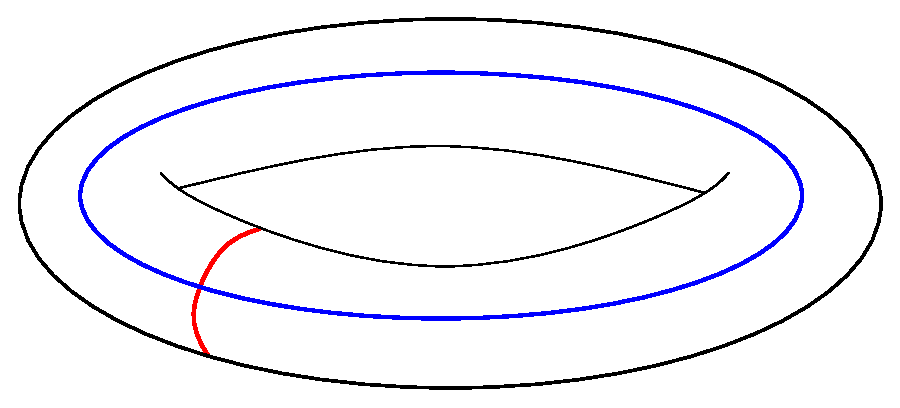
\includegraphics[width = \textwidth ]{figs/torus.eps}
		\caption{A torus has 2 possible non-contractible loops highlighted in red and blue. These loops can be formed from either X or Z Pauli operators.}
	\end{minipage}
	\caption{}
	
\end{figure}
An interesting characteristic of the toric code is that due to the dual-lattice nature, X and Z errors can be dealt with the same way, through the use of a Hadamard gate\footnote{See appendix \ref{app:hadamard}}. For conciseness, simulations were only performed with X errors. 
\\\\
The easy scalability of the toric code, and its position as the simplest topological code, make it both a central idea, and an important subject of study in regards to quantum error correction.
\\\\
In regards to figure \ref{fig:toricgrid}, an odd number of blue loops or an odd number of red loops, constitutes a logical error. This error is due to the loops forming homologically non-trivial topologies. If an even number of red, or an even number of blues loops are formed, then the topology that is formed is homologically trivial, and has no effect on encoded qubits. If a red and a blue loop form, then the resulting topology is also trivial, with no effect on the logical qubits. These trivial topologies mean that the topology of the surface (state of the qubit) is left unchanged. 
\\\\
To determine if the correction procedure was a success, the cycles $D = E+E'$ can be evaluated to check if the homology has changed. If the homology class of the cycle $D$ is non-trivial, then the code is no longer in the ground state, and encoded information has be changed\footnote{see appendix \ref{app:cycles} for more information on trivial/nontrivial cycles}. Errors form 1D chains taking the system out of its ground state, and into an orthogonal subspace. Correction procedures attempt to fix this by connecting chains into complete cycles. If the cycles that the correction procedure are homologically trivial, then the codespace gets mapped to itself in a non-trivial way, and the encoded information is lost. If the cycles are trivial however, then the information is protected.

Errors on the toric code are enacted through chains of Pauli operators, denoted as $E$. These chains preserve the code space if the chains of errors form cycles on the lattice. That is to say that the sites acted upon by Z operators must form cycles on the lattice, and sites acted upon by X's must form cycles on the dual lattice. 

Decoding the syndrome of the Toric Code consists of matching anyons (measurable end points of the error chains) together to create homologically trivial cycles. The correction path is denoted $E^\prime$.


\section{Random-Bond Ising model}
	Decoding the syndrome of the Toric Code for an uncorrelated error model was show by Dennis et al \cite{Dennis2001}, to be the same as solving the random-bond Ising model (RBIM) in 2D. The result of this work showed that optimal matching procedure for this error model is a least weight matching between syndrome measurements of -1. In this model, degenerate least weight paths have no effect. Recent studies by Stace and Barret \cite{Stace2010} and Dennis et al\cite{Dennis2001} have shown that the degeneracy of the matching path has an appreciable effect on the success rate of the code. The model implemented in this project however, ignores the effect of degeneracy, and chooses a random path from the degenerate matchings. This decoding step is shown in figure \ref{fig:graphicaloutput}, with a red error chain ($E$) and a yellow least weight path matching ($E^\prime$) the green anyons (Ising vorticies).
	
	\begin{figure}[htpb]
	\centering
	\includegraphics[width=0.5\textwidth ]{figs/graphicaloutput.png}
	\caption{A 5 by 5 torus. Blue dots indicate aligned regions ($\tau = +1$), red dots indicate unaligned ($\tau = -1$). The red lines show the one dimensional chains of antiferromagnetic bonds ($E$), which terminate in Ising vorticies (green dots). These Ising vorticies are then least weight matched ($E'$, in yellow).}
	\label{fig:graphicaloutput}
	\end{figure}
	
	This model is analogous to our treatment of a qubit prone to a single type of error. Spins in this model anti-align with probability $p$ and align with probability $1-p$. Spins that are align have the value $\tau_{ij}=+1$ and spins that anti-align take the value $\tau_{ij}=-1$. Again, if an odd number of spins in a plaquette have $\tau_{ij}= -1$, then that plaquette is the location of an Ising vortex, and analogously for star stabilizers.
	
	Applying the RBIM model can give new insights in possible ansatz with which to make predictions about how the code behaves. 

\section{Scaling}
	When using a least weight matching procedure derived from the RBIM model, the Toric code a has a critical error rate $p_{c0}$, below which large loops (more likely to be topologically nontrivial) are suppressed, and above which larger loops are promoted. This provides the toric code with a high chance of success below the threshold $p_{c0}$, and a low chance of success above the threshold. As $L\rightarrow \inf$ ; the transition between suppression and promotion of large loops leads to a discontinuity in $P_{success} \propto p$, where $P_{success}$ is the rate at which the encoded information is protected. This behaviour as the code scales with L can be described by the critical exponent $v_0$, and the critical point $p_c0$. The critical exponent characterizes that rate at which the average chain length (correlation length of the 1D chains) diverges from L. The relation between these values is shown in equation \ref{eq:scalingrelation}.
	
	\begin{equation}
	 x = (p-p_{c0})L^{1/v_0} 
	 \label{eq:scalingrelation}
	\end{equation}

	This relation allows us to map from 3 variables ($L$, $p$, $P_{success}$), into 2 ($x$, $P_{success}$), and lets us compare data between different code sizes (for sufficiently large L). The critical exponent and the critical point can be found experimentally. The critical point can be found by determining at what point lines of $P_{success} \propto p$ cross. The critical exponent can be found through variation, and optimizing for when the curves of $P_{success} \propto p$ are parallel. 

	The $E$ and $E^\prime$ are dependant upon L being even or odd. For this reason, we will find unique $v_0$ and $p_{c0}$ for the even and odd cases.
\section{Random Walks}
	\subsection{Random walks}
	Random walks can take several forms. 
	\begin{itemize}
		\item self avoiding random walk
		\item non-self avoiding 
		\item other variation $\cdots$ self flipping? non inverting or whatever.. have written in logbook...
	\end{itemize}
 	non-self avoiding random walks are the kind of error that this thesis investigates. 
 	This kind of random walk on a 2D grid has 4 possible moves at every timestep, and can move a distance of 1. 
 	These random walks can be characterized by their expected walk length. The expected walk length can take several forms.
 	By far the easiest to calculate walk length is the root-mean-square (RMS) walk length. This walk length is simply proportional to RMS of the number of steps. 
 	\begin{equation}
 	RMS(N) = \sqrt{N}s
 	 \end{equation}
 	The second type of distance, is the average Pythagorean distance. This distance is more complicated to calculate, and is found through the equation \ref({eq:pythag}
 	
 	Expected Pythagorean distance:
 	\begin{equation}
 	D(N) = \frac{1}{4^N}\sum_{i=0}^{N}\sum_{j=0}^{N}\prescript{N}{}{C}_{i}\prescript{N}{}{C}_{j} \frac{1}{\sqrt{2}}\sqrt{(2i-N)^2+(2j-N)^2)} 
 	\end{equation}
 	
 	Expected Manhattan distance:
 	\begin{equation*}
 	D(N) = \frac{1}{4^N}\sum_{i=0}^{N}\sum_{j=0}^{N}\prescript{N}{}{C}_{i}\prescript{N}{}{C}_{j} \frac{1}{\sqrt{2}} 
 	\begin{bmatrix}
 	1&1\\
 	\end{bmatrix} 
 	\left|
 	\begin{bmatrix}
 	\frac{1}{\sqrt{2}} & \frac{1}{\sqrt{2}} \\
 	\frac{-1}{\sqrt{2}} & \frac{1}{\sqrt{2}} 
 	\end{bmatrix}
 	\begin{bmatrix}
 	2i-N \\
 	2j-N
 	\end{bmatrix}
 	\right|
 	\end{equation*}
 	
	These formulas line up well with plots made from the distributions of simulated walks. 
	Figure \ref{fig:dists} shows how these mean values compare to the shape of the distributions. Figure \ref{fig:dists} shows gamma functions fitted to data of the manhattan distance and the pythagorean distances of the end points of 10,000 random walks. 
	
	\begin{figure}
		\centering
		\includegraphics[width = 0.8\textwidth]{figs/randomwalkdistribution_1000000_32}
		\label{fig:randomwalkdistributions}
		\caption{This figure is a PDF of the distance of generated random walks, with the distance calulated in different ways}
	\end{figure}
	important walklengths in figure \ref{fig:randomwalkdistributions} are the three calculated mean distances, and the locations of the turning points for the gamma distributions. 
	\begin{table}
	\centering
	\begin{tabular}{c c}
	Manhatten expected&  6.358192239869876\\ 
	Pythagorean expected&  5.016712342283284\\ 
	$\sqrt{N}$ &  5.6568542494923806\\ 
	Pythagoren PDF TP &  4.2506712139429359\\ 
	Manhattan PDF TP &  5.1970956125713439\\ 
	\end{tabular} 
	\caption{Important points from the PDFs for a walk length of N=32. }
	\label{tab:candidates}
	\end{table}
	The points in table \ref{tab:candidates} are potential candidate parameters for correction functions for correlated error models. 

 	The probability density function (PDF) in figure \ref{fig:randomwalkdistributions} were generate using Markov Chain Monte Carlo (MCMC) methods. These PDFs were then used to create a more accurate correction function for the Toric Code, as when we know that the distribution looks like figure \ref{fig:randomwalkdistributions} rather than an exponential decay (as in the non-correlated model), we can conclude that correcting proportionally to this distribution, rather than as simply a linear scale with distance; we should see an improved success rate of the code. 
 
 \subsection{Random walks again}
The distribution of random walks was shown by Lord Rayleigh \cite{bibid} to be approximated by the Rayleigh equation for diffusion for large step sizes. Computationally, large step sizes are very hard to compute for large samples of random walks. Here we develop exact solutions for random walks, to determine the expected walk length of a random walk after $N$ steps. We determine the expected walk length in terms of the Manhattan distance, and the Pythagorean distance, as both are of importance to the match scheme for correlated errors on the Toric code. We shall then confirm the results of these equations to the PDFs of simulated random walks, and the Rayleigh equation for diffusion. 

Firstly, the Rayleigh equation for diffusion:
\begin{equation}
P_N(R) \sim \frac{2R}{N}e ^{-R^2/N}
\label{eq:rayleigh}
\end{equation}
In 1906 Rayleigh proposed a method to calculate the PDF of a random walk for large N \cite{Rayleigh1905}. Here we show an exact method for determining the expected walk length; which is useful for our purposes of creating a correction function based upon a gaussian centred at that distance.  

\begin{align}
P_N(L) & = \frac{\sum_{i\in \mathds{S}}\sum_{j\in \mathds{S}} {}^NC_i {}^NC_j - \sum_{i\in \mathds{P}}\sum_{j\in \mathds{P}} {}^NC_i {}^NC_j}
{\sum_{i = 0}^N\sum_{j=0}^N {}^NC_i {}^NC_j }\\
\label{eq:exactPDF}
\end{align}
Where 
\begin{align}
\centering
	\mathds{S} &= \{ \frac{N-L}{2} \leq n \leq \frac{N+L}{2};  \hspace{1cm} n\in \mathds{Z}^{even} \}\\
	\mathds{P} &= \{\frac{N-L}{2}+1 \leq n \leq \frac{N+L}{2}-1;  \hspace{1cm} n\in \mathds{Z}^{even}\}
\end{align}
Where we define the sum of a null set to be zero. 


\begin{figure}
\centering
\includegraphics[width = 0.7\textwidth]{figs/calculatedvssimulated.pdf}
\caption{A comparison of the calulated values vs simulated walk data for 1,000,000 random walks. RMS error between the two trends was 7e-06. }
\label{fig:exactproof}
\end{figure}
Figure \ref{fig:exactproof} shows excellent agreement of formula \ref{eq:exactPDF} to walk data. 



\begin{figure}
\centering
\includegraphics[width = 0.7\textwidth]{figs/exactPDF.pdf}
\caption{This figure shows the exact PDF calculated for walks of various lengths. This data is generated from equation \ref{eq:exactPDF}.}
\end{figure}







\section{Correlated Errors}
	The recovery process (pairwise matching) is shown to be most effective when it is least weight \cite{Dennis2001}. Least weight matching is however only true for uncorrelated errors.
	Correlated errors can arise when nearby qubits are not well isolated from one anther, and this can allow errors to `walk' from qubit to qubit.

 	\subsection{Correlated errors}

	In the case of correlated errors, matchings that are similar in length to the average length of a random walk are more preferential for successful matchings. This length of walk can be used to improve the recovery process. The correlation length that the recovery process optimizes for can either be fixed, or can be adaptive as an ancilla memory gains information about the system. Information from the syndrome can be used to determine the correlation length and improve the code over time. 
	\\\\
	The schematic (figure \ref{fig:schematic}) shows how this toric code can then be used to feedback information over many cycles to store knowledge about the errors and to improve its correction rate over time. Information about error gained from the syndrome measurements can be stored in ancilla qubits, for use in `training' the decoder to optimally decode correlated errors.
	
	\begin{figure}[htpb]
	\centering
	\includegraphics[width =0.8\textwidth]{figs/schematic.eps}
	\caption{The logical qubits are encoded into the Toric code as $2$ logical qubits onto $2L^2$ physical qubits. These qubits then pass through an error channel. The syndrome is then measured, and an appropriate correction procedure takes place. The code is then decoded, and checked for success. }
	\label{fig:schematic}
	\end{figure}


